\section{Generalized Cross Correlation}
\label{sec:02_gcc}

As depict in \cref{sec:02_cc}, the \ac{CC} can bring some error sources in the context of
incorrect delay results and inaccuracy.
Improvements were done in research by introducing prefilters for the signals
which is equal to general frequency weighting as stated in \cite{K_C_GCC}.
\begin{figure}[ht]
	\centering
		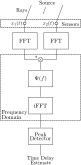
\includegraphics[width=0.35\columnwidth]{figures/GCC_weight}
	\caption{Generalized cross correlation for time delay estimation}
    \label{fig:02_GCC}
\end{figure}
With certain weightings $H_i(f)$ prior to the \ac{CC}, the peak detection
can be rectified by improving the relation between peak and noise or
enhancing the accuracy \cite{H_B_GCC}.
Figure \cref{fig:02_GCC} illustrates the process of a \ac{GCC} with both filters combined as
$\Psi(f) = H_1^*(f)H_2$. The figure in \cref{appendix:a1_alternativeGcc} represents the
\ac{GCC} with $H_i(f)$.
After transforming the signals $x_i(f)$ into frequency domain, the cross correlated
signals are multiplied with the weighting $\Psi(f)$ and transformed back into time domain.
The subsequent steps are similar to the \ac{CC}.

Thus, the \ac{GCC} is declared as
\bsub
\bal
    R^{(g)}_{x_1x_2}(t) &= \int^{+\infty}_{-\infty}\Psi(f)G_{x_1x_2}(f)e^{j2\pi ft} df.
    \label{eq:02_gcc}\\
\intertext{Written-out it is visible how the choice of $\Psi(f)$ impacts the individual segments of \cref{eq:02_Gx1x2}
as}
    R^{(g)}_{x_1x_2}(f) &= \mathcal{F}^{-1}[\Psi(f) \alpha \phi_s(f) e^{-j2\pi fD}] \nonumber \\
    &+ \mathcal{F}^{-1}[\Psi(f) \phi_n(f)] + \mathcal{F}^{-1}[\Psi(f) \phi_c(f)].
    \label{eq:02_gcc_long}
\eal
\esub
Several variants of the weighting were designed by various researchers with different criteria.
They have in common, that they take the characteristics of the received signals into account.
Some favor one of both signals, some are designed to suppress the noise and other focus to
sharpen the peak as contrasted in \cite{K_C_GCC}.
The characteristics of the \ac{GCC} with \ac{PHAT} most appealed to the task in this work and
is chosen as weighting function.
% -------------------------------------------------------------
\subsection{The Phase Transform (PHAT)}
The \ac{PHAT} weighting is known as
\bal
    \Psi^{(P)}(f) = \frac{1}{|G_{x_1x_2}(f)|}.
\eal
For the ideal case that $\phi_n$ and $\phi_c$ are nonexistent due to non-correlation,
the the \ac{GCC} results in
\bal
    R^{(p)}_{x_1x_2}(t) = \mathcal{F}^{-1}[\frac{\alpha |S(f)|^2 e^{-j2\pi fD}}{|G_{x_1x_2}(f)|}] = \delta(t-D)
\eal
because $|G_{x_1x_2}(f)| = \alpha |S(f)|^2$.
This filter is used regularly in research, due to the characteristic of sharpening
the peak what leads in high accuracy.
% -------------------------------------------------------------

Figure \cref{fig:03_gccTheory} shows the result of the \ac{GCC-PHAT} algorithm with a generated
simple Hann-windowed signal as input. Both signals are 3000\si{Hz} sine signals, whereby
the second signal is shifted by 10 samples.
The signals are similar to the ones used in \cref{sec:02_cc}
and are plotted in \cref{sec:abbreviations}.
Compared to the \ac{CC} in \cref{sec:02_cc}, the sharp peak is distinct.
However, \cite{K_C_GCC} complains about the lower robustness of this algorithm.
\begin{figure}[ht]
	\centering
		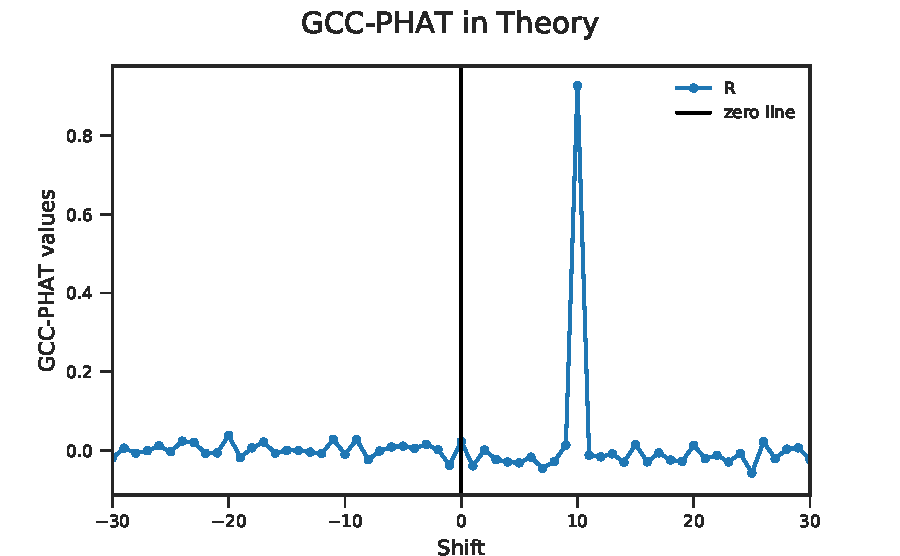
\includegraphics[width=1\columnwidth]{figures/GCC_theory}
	\caption{Generalized Cross Correlation with PHAT weighting of two generated 3000Hz sine signals.}
    \label{fig:03_gccTheory}
\end{figure}

%- whistle frequency between 2000Hz and 4000Hz (low-pass)\\
%- thus, the peaks of the cross-correlation are wide\\